% Created 2019-09-12 Thu 15:20
% Intended LaTeX compiler: pdflatex
\documentclass[sigplan,screen]{acmart}
\usepackage[utf8]{inputenc}
\usepackage[T1]{fontenc}
\usepackage{graphicx}
\usepackage{grffile}
\usepackage{longtable}
\usepackage{wrapfig}
\usepackage{rotating}
\usepackage[normalem]{ulem}
\usepackage{amsmath}
\usepackage{textcomp}
\usepackage{amssymb}
\usepackage{capt-of}
\usepackage{hyperref}
\usepackage{minted}
\usepackage{edcomms}
\edcommsfalse
\usepackage[font=itshape]{quoting}
\pdfpagewidth=8.5in
\pdfpageheight=11in
\usepackage{color}
\definecolor{darkgreen}{rgb}{0.0, 0.3, 0.1}
\hypersetup{colorlinks,linkcolor=darkgreen,citecolor=darkgreen,urlcolor=darkgreen}
\usepackage{CheatSheet/UnicodeSymbols}
\DeclareMathOperator{\VCCompose}{\longrightarrow\hspace{-3ex}\oplus\;}
\newunicodechar{⟴}{\ensuremath{\!\!\VCCompose}}
\newunicodechar{𝓋}{\ensuremath{\!\!v}}
\newunicodechar{𝒱}{\ensuremath{\mathcal{V}}}
\newunicodechar{α}{\ensuremath{\alpha}}
\newunicodechar{𝑛}{\ensuremath{n}}
\newunicodechar{𝑎}{\ensuremath{a}}
\newunicodechar{𝑚}{\ensuremath{m}}
\newunicodechar{𝑒}{\ensuremath{e}}
\newunicodechar{⁰}{\ensuremath{^0}}
\newunicodechar{³}{\ensuremath{^3}}
\clubpenalty = 10000
\widowpenalty = 10000
\displaywidowpenalty = 10000
\usepackage{flushend}
\setcopyright{acmcopyright}
\acmPrice{15.00}
\acmDOI{10.1145/3357765.3359523}
\acmYear{2019}
\copyrightyear{2019}
\acmISBN{978-1-4503-6980-0/19/10}
\acmConference[GPCE '19]{Proceedings of the 18th ACM SIGPLAN International Conference on Generative Programming: Concepts and Experiences}{October 21--22, 2019}{Athens, Greece}
\acmBooktitle{Proceedings of the 18th ACM SIGPLAN International Conference on Generative Programming: Concepts and Experiences (GPCE '19), October 21--22, 2019, Athens, Greece}
\date{\today}
\title{A Language Feature to Unbundle Data at Will (Short Paper)}
\hypersetup{
 pdfauthor={Musa Al-hassy},
 pdftitle={A Language Feature to Unbundle Data at Will (Short Paper)},
 pdfkeywords={},
 pdfsubject={Thesis proposal for Musa Al-hassy; McMaster University 2019.},
 pdfcreator={Emacs 26.1 (Org mode 9.2.5)},
 pdflang={English}}
\begin{document}




\settopmatter{printacmref=false, printccs=true, printfolios=false}


%%
%% The code below is generated by the tool at http://dl.acm.org/ccs.cfm.

\begin{CCSXML}
<ccs2012>
<concept>
<concept_id>10011007.10011006.10011008.10011009.10011019</concept_id>
<concept_desc>Software and its engineering~Extensible languages</concept_desc>
<concept_significance>500</concept_significance>
</concept>
<concept>
<concept_id>10011007.10011006.10011008.10011024.10011031</concept_id>
<concept_desc>Software and its engineering~Modules / packages</concept_desc>
<concept_significance>500</concept_significance>
</concept>
<concept>
<concept_id>10011007.10011006.10011008.10011009.10011012</concept_id>
<concept_desc>Software and its engineering~Functional languages</concept_desc>
<concept_significance>300</concept_significance>
</concept>
<concept>
<concept_id>10011007.10011006.10011008.10011024.10011025</concept_id>
<concept_desc>Software and its engineering~Polymorphism</concept_desc>
<concept_significance>300</concept_significance>
</concept>
<concept>
<concept_id>10011007.10011006.10011008.10011024.10011028</concept_id>
<concept_desc>Software and its engineering~Data types and structures</concept_desc>
<concept_significance>300</concept_significance>
</concept>
<concept>
<concept_id>10011007.10011006.10011041.10011047</concept_id>
<concept_desc>Software and its engineering~Source code generation</concept_desc>
<concept_significance>300</concept_significance>
</concept>
<concept>
<concept_id>10011007.10011006.10011060.10011018</concept_id>
<concept_desc>Software and its engineering~Design languages</concept_desc>
<concept_significance>300</concept_significance>
</concept>
<concept>
<concept_id>10011007.10011006.10011066.10011069</concept_id>
<concept_desc>Software and its engineering~Integrated and visual development environments</concept_desc>
<concept_significance>300</concept_significance>
</concept>
<concept>
<concept_id>10011007.10011006.10011008.10011009.10011010</concept_id>
<concept_desc>Software and its engineering~Imperative languages</concept_desc>
<concept_significance>100</concept_significance>
</concept>
<concept>
<concept_id>10011007.10011006.10011008.10011024.10003202</concept_id>
<concept_desc>Software and its engineering~Abstract data types</concept_desc>
<concept_significance>100</concept_significance>
</concept>
<concept>
<concept_id>10011007.10011006.10011008.10011024.10011036</concept_id>
<concept_desc>Software and its engineering~Patterns</concept_desc>
<concept_significance>100</concept_significance>
</concept>
<concept>
<concept_id>10011007.10011006.10011039.10011040</concept_id>
<concept_desc>Software and its engineering~Syntax</concept_desc>
<concept_significance>100</concept_significance>
</concept>
</ccs2012>
\end{CCSXML}

\ccsdesc[500]{Software and its engineering~Extensible languages}
\ccsdesc[500]{Software and its engineering~Modules / packages}
\ccsdesc[300]{Software and its engineering~Functional languages}
\ccsdesc[300]{Software and its engineering~Polymorphism}
\ccsdesc[300]{Software and its engineering~Source code generation}
\ccsdesc[300]{Software and its engineering~Integrated and visual development environments}

%removed
\ccsdesc[300]{Software and its engineering~Data types and structures}
\ccsdesc[300]{Software and its engineering~Design languages}
\ccsdesc[100]{Software and its engineering~Imperative languages}
\ccsdesc[100]{Software and its engineering~Patterns}
\ccsdesc[100]{Software and its engineering~Syntax}
\ccsdesc[100]{Software and its engineering~Abstract data types}


%%
%% Keywords. The author(s) should pick words that accurately describe
%% the work being presented. Separate the keywords with commas.
\keywords{Agda, meta-program, extensible, Emacs, pacakges, modules, dependent-types}

 \title{A Language Feature to Unbundle Data at Will}
\subtitle{ (Short Paper)}

 \author{Musa Al-hassy}
 \affiliation{McMaster University, Canada}
 \email{alhassy@gmail.com}

 \author{Jacques Carette}
 \orcid{0000-0001-8993-9804}
 \affiliation{McMaster University, Canada}
 \email{carette@mcmaster.ca}

 \author{Wolfram Kahl}
 \orcid{0000-0002-6355-214X}
 \affiliation{McMaster University, Canada}
 \email{kahl@cas.mcmaster.ca}

 % \author{Musa Al-hassy \\ {\small \url{alhassy@gmail.com} \\ McMaster University \\ Computing and Software \\ Hamilton, Ontario, Canada}}
 % \author{Jacques Carette \\ {\small \url{carette@mcmaster.ca} \\ McMaster University \\ Computing and Software \\ Hamilton, Ontario, Canada}}
 % \author{Wolfram Kahl \\ {\small \url{kahl@cas.mcmaster.ca} \\ McMaster University \\ Computing and Software \\ Hamilton, Ontario, Canada}}



\begin{abstract}


Programming languages with sufficiently expressive type systems provide users with
different means of data ‘bundling’. Specifically, in dependently-typed languages such as
Agda, Coq, Lean and Idris, one can choose to encode information
in a record either as a parameter or a field.
For example, we can speak of graphs \emph{over} a particular vertex set, or speak
of arbitrary graphs where the vertex set is a component.
These create isomorphic types, but differ with respect to intended use.
Traditionally, a library designer would make this choice (between parameters and fields);
if a user wants a different variant, they are forced to build conversion utilities, as well as
duplicate functionality. For a graph data type,
if a library only provides a Haskell-like typeclass view of graphs \emph{over} a vertex set,
yet a user wishes to work with the category of graphs, they must now package a vertex
set as a component in a record along with a graph over that set.

We design and implement a language feature that allows both the library designer and
the user to make the choice of information exposure only when necessary, and otherwise leave
the distinguishing line between parameters and fields unspecified.
Our language feature is currently implemented as a prototype meta-program
incorporated into Agda's Emacs ecosystem, in a way that is unobtrusive to Agda users.
\end{abstract}

\maketitle

\section{Introduction --- Selecting the ‘Right’ Perspective}
\label{sec:orgfe4751e}

Library designers want to produce software components that are useful for
the perceived needs of a variety of users and usage scenarios.  It is therefore
natural for designers to aim for substantial generality, in the hopes of increased
reusability. One such particular ``choice'' will occupy us here: When creating a
record to bundle up certain information that “naturally” belongs together, what
parts of that record should be \emph{parameters} and what parts should be
\emph{fields}? This is analogous to whether functions are curried and so arguments
may be provided partially, or otherwise must be provided all-together in one tuple.

The subtlety of what is a ‘parameter’ --- exposed at the type level --- and what is a
‘field’ --- a component value --- has led to awkward formulations and
the duplication of existing types for the sole purpose of different uses.
Tom Hales \cite{Hales-blog-post} is quite eloquent in his critique of Lean:
\begin{quoting}
 Structures are meaninglessly parameterized from a mathematical perspective.
 [\ldots{}] I think of the parametric versus bundled variants as analogous to currying
 or not; are the arguments to a function presented in succession or as a single
 ordered tuple? However, there is a big difference between currying functions
 and currying structures. Switching between curried and uncurried functions is
 cheap, but it is nearly impossible in Lean to curry a structure. That is, what
 is bundled cannot be later opened up as a parameter. (Going the other direction
 towards increased bundling of structures is easily achieved with sigma types.)
This means that library designers are forced to take a conservative approach and
expose as a parameter anything that any user might reasonably want exposed, because
once it is bundled, it is not coming back.
\end{quoting}
This is the problem we are solving.

For example, each Haskell typeclass can have only one instance per datatype;
since there are several monoids with the datatype \texttt{Bool} as carrier,
in particular those induced by conjunction and disjunction,
the de-facto-standard libraries for Haskell
define two isomorphic copies \texttt{All} and \texttt{Any} of \texttt{Bool},
only for the purpose of being able to attach the respective monoid instances to them.

But perhaps Haskell's type system does not give the programmer sufficient
tools to adequately express such ideas. As such, for the rest of this paper
we will illustrate our ideas in Agda \cite{Norell-2007,agda_overview}.
For the monoid example,
it seems that there are three contenders for the monoid interface:

\noindent
\begin{minted}[]{agda}
  record Monoid₀ : Set₁ where
    field
      Carrier : Set
      _⨾_     : Carrier → Carrier → Carrier
      Id      : Carrier
      assoc   : ∀ {x y z}
              → (x ⨾ y) ⨾ z ≡ x ⨾ (y ⨾ z)
      leftId  : ∀ {x} → Id ⨾ x ≡ x
      rightId : ∀ {x} → x ⨾ Id ≡ x

  record Monoid₁ (Carrier : Set) : Set where
    field
      _⨾_     : Carrier → Carrier → Carrier
      Id      : Carrier
      assoc   : ∀ {x y z}
              → (x ⨾ y) ⨾ z ≡ x ⨾ (y ⨾ z)
      leftId  : ∀ {x} → Id ⨾ x ≡ x
      rightId : ∀ {x} → x ⨾ Id ≡ x

  record Monoid₂
           (Carrier : Set)
           (_⨾_ : Carrier → Carrier → Carrier)
         : Set  where
    field
      Id      : Carrier
      assoc   : ∀ {x y z}
              → (x ⨾ y) ⨾ z ≡ x ⨾ (y ⨾ z)
      leftId  : ∀ {x} → Id ⨾ x ≡ x
      rightId : ∀ {x} → x ⨾ Id ≡ x
\end{minted}

\vspace{0.3em}\noindent
In \texttt{Monoid₀}, we will call \texttt{Carrier} “bundled up”,
while we call it “exposed” in \texttt{Monoid₁} and \texttt{Monoid₂}.
The bundled-up version allows us to speak of \emph{a}
monoid, rather than \emph{a monoid on a given type} which is captured by \texttt{Monoid₁}.
While \texttt{Monoid₂} exposes both the carrier and the composition operation,
we might in some situation be interested
in exposing the identity element instead
--- e.g., the discrepancy ‘≢’ and indistinguishability ‘≡’ operations
on the Booleans
have the same identities as conjunction and disjunction, respectively.
Moreover, there are other combinations of what is to be exposed and hidden,
for applications that we might never think of.

Rather than code with \emph{interface formulations we think people will likely use}, we can
instead try to \emph{commit to no particular formulation} and allow the user to select
the form most convenient for their use-cases. This desire for reusability motivates
a new language feature: The \textsf{\upshape PackageFormer}.

Moreover, it is often the case that one begins working with a record of useful
semantic data, but then, say, for proof automation, may want to use the associated
datatype for syntax. For example, the syntax of closed monoid terms can be expressed,
using trees, as follows.
\begin{minted}[]{agda}
    data Monoid₃ : Set where
      _⨾_ : Monoid₃ → Monoid₃ → Monoid₃
      Id  : Monoid₃
\end{minted}
\noindent
We can see that this can be
obtained from \texttt{Monoid₀} by discarding the
fields denoting equations, then turning the remaining fields into constructors.

We show how these different
presentations can be derived from a \emph{single}
\textsf{\upshape PackageFormer} declaration
via a generative meta-program integrated into the
most widely-used Agda “IDE”, the Emacs mode for Agda.
In particular,
if one were to explicitly write \(M\) different bundlings of a package
with \(N\) constants then one would write nearly \(N × M\) lines of code,
yet this quadratic count becomes linear \(N + M\) by having a single
package declaration of \(N\) constituents with \(M\) subsequent instantiations.
We hope that reducing such duplication of effort, and of potential maintenance
burden, will be beneficial to the software engineering of large libraries
of formal code --- and consider it the main contribution of our work.

\section{\textsf{\upshape PackageFormer}s --- Being Non-committal as Much as Possible}
\label{sec:orgc0c4ed5}
We claim that the above monoid-related pieces of Agda code
can be unified as a single declaration
which does not distinguish between parameters and fields,
where \texttt{PackageFormer} is a keyword with similar syntax as \texttt{record}:

\begin{minted}[]{agda}
  PackageFormer MonoidP : Set₁ where
    Carrier : Set
     _⨾_    : Carrier → Carrier → Carrier
    Id      : Carrier
    assoc   : ∀ {x y z}
            → (x ⨾ y) ⨾ z ≡ x ⨾ (y ⨾ z)
    leftId  : ∀ {x} → Id ⨾ x ≡ x
    rightId : ∀ {x} → x ⨾ Id ≡ x
\end{minted}

\noindent

 Then, with various directives that let one declare
 what should be parameters and what should be fields,
 we can reproduce the above presentations.
The directives can be built from the following grammar:
\begin{minted}[]{agda}
  id          :  Variational
  record      :  Variational
  typeclass   :  Variational
  termtype    :  String → Variational
  unbundled   :  ℕ → Variational
  exposing    :  List Name → Variational
  _⟴_        :  Variational
              →  Variational → Variational
\end{minted}

\noindent
  A package former is used via \emph{instantiations}, written as low-precedence
 juxtapositions of a package former name and expression of type
 \texttt{Variational}.
 Notice that some variationals have arguments.
 For example, \texttt{exposing} explicitly lists the names that should be turned
 into parameters, in that sequence, \texttt{“unbundled} \(n\)” exposes the
 first \(n\) names declared in the package former.

An \emph{instantiation} juxtaposition is written \texttt{PF 𝓋} to indicate that the PackageFormer
named \texttt{PF} is to be restructred according to scheme \(\hspace{1ex}\!\) \texttt{𝓋}. A \emph{composition} of variationals
is denoted using the symbol ‘⟴’; for example,
\begin{center}
\texttt{PF 𝓋₁ ⟴ 𝓋₂ ⟴ ⋯ ⟴ 𝓋ₙ}
\end{center}
\noindent
 denotes the forward-composition of iterated instantiations,
 namely ((\texttt{(PF 𝓋₁) 𝓋₂) ⋯) 𝓋ₙ}, since we take prefix instantiation application
to have lower precedence that variational composition.
 In particular, an empty composition is the identity
 scheme, which performs no alteration, and has the explicit name \texttt{id}.
 Since \(\mathsf{PF} \; \mathsf{id} ≈ \mathsf{PF}\) and \texttt{id} is the identity of composition, we may
 write any \emph{instantiation} as a sequence of \hspace{0.2em} ⟴-separated clauses:
\begin{center}
\texttt{PF ⟴ 𝓋₁ ⟴ 𝓋₂ ⟴ ⋯ ⟴ 𝓋ₙ}
\end{center}

The previous presentations can be obtained as follows.

\begin{enumerate}
\setcounter{enumi}{-1}
\item To make \texttt{Monoid₀′} the type of \emph{arbitrary monoids}
(that is, with arbitrary carrier), we declare:
\vspace{0.3em}
\begin{verbatim}
 Monoid₀′  = MonoidP record
\end{verbatim}

\setcounter{enumi}{0}
\item We may obtain the previous formulation of
\texttt{Monoid₁} in two different equivalent ways:
\vspace{0.3em}
\begin{verbatim}
 Monoid₁′  = MonoidP record ⟴ unbundled 1
 Monoid₁″ = Monoid₀′ exposing (Carrier)
\end{verbatim}

\vspace{0.3em}
It is interesting to note that \emph{PackageFormer} \texttt{MonoidP} is treated on the same footing
\emph{record} \texttt{Monoid₀′}: Both may be subjected to variationals.
\end{enumerate}

\begin{enumerate}
\setcounter{enumi}{1}
\item As with \texttt{Monoid₁}, there are also different ways
to obtain \texttt{Monoid₂}.
\vspace{0.3em}
\begin{verbatim}
 Monoid₂′  = MonoidP record ⟴ unbundled 2
 Monoid₂″ = Monoid₀′ exposing (Carrier; _⨾_)
\end{verbatim}

\vspace{0.3em}
\end{enumerate}

\begin{enumerate}
\setcounter{enumi}{2}
\item Metaprogramming is clearly needed to produce the term language:
\vspace{0.3em}
\begin{verbatim}
 Monoid₃′ = MonoidP termtype "Carrier"
\end{verbatim}
\vspace{0.3em}
\noindent
Our running example uses the theory of monoids, which is a single-sorted theory.
In general, a PackageFormer may have multiple sorts ---as is the case with
graphs--- and so one of the possibly many sorts needs to be designated as the
universe of discourse, or carrier, of the resulting inductively defined term type.
Such a purpose is served by the single argument to \texttt{termtype}.

\vspace{0.3em}
\noindent
We may also want to have terms \emph{over} a particular variable set, and so declare:
\vspace{0.3em}
\begin{verbatim}
 Monoid₄ = MonoidP
           termtype-with-variables "Carrier"
\end{verbatim}
\vspace{0.3em}
\noindent
Since a parameter's name does not matter, due to α-equivalence, an arbitrary,
albeit unique, name for the variable set is introduced along with an embedding
function from it to the resulting term type. For brevity, the embedding function's
name is \texttt{inj} and the user must ensure there is no name clash.
The resulting elaboration is as follows.
\vspace{0.3em}
\noindent
\begin{minted}[]{agda}
    data Monoid₄ (Vars : Set) : Set where
      inj : Vars → Monoid₄ Vars
      _⨾_ : Monoid₄ Vars
          → Monoid₄ Vars → Monoid₄ Vars
      Id  : Monoid₄ Vars
\end{minted}

\vspace{0.3em}
\noindent
Note that these instantiations implicitly drop equations, such
as associativity from \texttt{MonoidP}.  This is what is commonly done
in Universal Algebra. If we were instead doing \emph{n}-category
theory, these would be kept, but will be the subject of future
work.
\end{enumerate}

We also have elaborations into nested dependent-sums, which is useful
when looking at coherent substructures.
Alongside \texttt{unbundled}, we also have infix combinators for extending an
instantiation with additional fields or constructors, and the renaming of constituents
according to a user provided String-to-String function.
Moreover, just as syntactic datatype declarations may be derived, we also
allow support for the derivation of induction principles and structure-preserving homomorphism types.
Our envisioned system would be able to derive simple, tedious, uninteresting concepts; leaving difficult,
interesting ones for humans to solve.

\begin{quote}
\textbf{Quadratic to Linear:}
Notice that the previous 5 monoid presentations, \texttt{Monoid₀} to \texttt{Monoid₄}, spanned 32
lines (8 for the original, 24 for the variants). Using \texttt{MonoidP} and our operators,
this can be done in 7 + 6 = 13 lines.  This corresponds to using a 2-part code,
with the initial lines being a model, and then 1-2 lines to specify variants.
\end{quote}

\section{\textsf{\upshape Variational} Polymorphism}
\label{sec:org41e7204}
Suppose we want to produce the function \texttt{concat}, which folds over the elements of a list
according to a compositionality scheme --- examples of this include summing over
a list, multiplication over a list, checking all items in a list are true, or
at least one item in the list is true.
Depending on the selected instantiation,
the resulting function may have types such as the following:

\begin{minted}[]{agda}
  concat₀ : {M : Monoid₀}
          → let C = Monoid₀.Carrier M
             in  List C → C

  concat₁ : {C : Set} {M : Monoid₁ C}
          → List C → C

  concat₂ : {C : Set} {_⨾_ : C → C→ C}
            {M : Monoid₂ C _⨾_}
          → List C → C

  concat₃ : let C = Monoid₃
             in List C → C
\end{minted}

\noindent
Given our previous work, and providing that the variationals are already
defined, we add a new declaration which, unlike the rest, comes
equipped with a \emph{definition}.
\vspace{0.3em}
\begin{minted}[]{agda}
    concat : List Carrier → Carrier
    concat = foldr _⨾_ Id
\end{minted}
\noindent
This is known as a \emph{definitional extension} (of a theory), which
is known to be conservative (i.e. has the same models).

The variationals is where this power comes from.  Furthermore, we have alluded to
the fact that the type of variationals
is extensible; this is achieved by having
\begin{center}
\texttt{Variational ≅ (PackageFormer → PackageFormer)}
\end{center}
\noindent
Indeed, our implementation relies on 5 meta-primitives to form arbitrarily
complex schemes that transform abstract PackageFormers into
other grouping mechanisms. The meta-primitives were arrived at by codifying
a number of structuring mechanisms directly then carefully extracting the minimal
ingredients that enable them to be well-defined.

\section{How Does This Work?}
\label{sec:org3843ed7}

We have implemented our system as an “editor tactic” meta-program.

In actual use, an Agda programmer declares what they want
using the combinators above (inside special Agda code comments).
The comments are read by Emacs Lisp and legitimate Agda is produced in a generated file, which is
then automatically imported into the current file --- examples are provided in an appendix.
The generated file never needs to be consulted,
as the declared names are furnished with tooltips rendering the elaborated
Agda form. Moreover, we also provide a feature to extract a ‘bare bones’ version
of a file that strips out all PackageFormer annotations, leaving only Agda
as well as the import to the generated file. Finally, since the elaborations are
just Agda, one only needs to use the system once and future users are
not forced to know about it.

The existing prototype already has the following nice properties:
\begin{description}
\item[{Extensible}] Users may extend the collection of variationals by providing the intended
elaboration scheme.

We have provided a number of auxiliary, derived, combinators
that can be used to construct complex and common schemes.
Furthermore, the user has full and direct access to the entirety of Emacs Lisp
as a programming language for restructuring PackageFormers into any desired shape
---the well-formedness of which is a matter the user must then worry about.

\item[{Practical}] The user manual demonstrates how boilerplate code for
            renamings, hidings, decorations, and generations
of hierarchical structures can be formed; \newline
\cite{tpc}.

\item[{Pragmatic}] The prototype comes equipped with a number of menus
to display the abstract PackageFormer's defined,
as well as the variationals defined, and one may
enable highlighting for these syntactical items, have
folded away, or simply extract an Agda file that does not mention
them at all.

As it can be tedious to consult generated code for high-level
PackageFormer instantiations and so every variational and PackageFormer
is tagged with tooltips providing relevant information.
\end{description}

\begin{figure}[htbp]
\centering
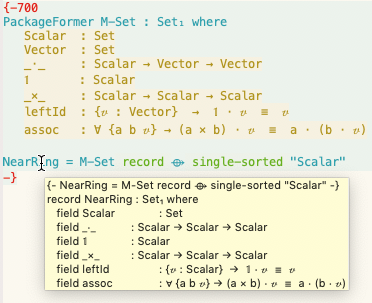
\includegraphics[width=.9\linewidth]{./Paper0_MousingOver.png}
\caption{Hovering to show details. Notice special syntax has default colouring: Red for PackageFormer delimiters, yellow for elements, and green for variationals.}
\end{figure}

\noindent
The details of the implementation and numerous common structuring mechanisms
derived from the meta-primitives can be found on the prototype's homepage:
\begin{center}
\url{https://alhassy.github.io/next-700-module-systems-proposal/prototype/PackageFormer.html}
\end{center}

\section{Next Steps}
\label{sec:orgcf66414}
We have outlined a new language feature that is intended to reduce
duplicated effort involved in taking different perspectives on structures---and to solve
Hales' problem of premature commitment to a particular encoding. Moreover, on the road
to making this tractable, we have unearthed a novel form of polymorphism and demonstrated
its usefulness with some examples.

We have presented our work indirectly by using examples, which we
hope are sufficiently clear to indicate our intent. We next intend to
provide explicit (elaboration) semantics for \texttt{PackageFormer} within a
minimal type theory; \newline \cite{types_for_modules}.

Furthermore, there are additional pieces of future work, including:

\begin{enumerate}
\item Explain how generative modules \cite{modular_modules}
are supported by this scheme.

\item How do multiple default, or optional, clauses for a constituent fit into this
language feature.

\item Explore inheritance, coercion, and transport along canonical isomorphisms.
\end{enumerate}

\noindent
Finally, the careful reader will have noticed
that our abstract mentions graphs, yet
there was no further discussion of that example.
We have avoided it for simplicity;
the prototype accommodates multi-sorted structures where
sorts may \emph{depend} on one another, as edge-sets
depend on the vertex-set chosen. Examples can be found on the prototype's
webpage.

This short paper proposes a language feature that enables users to selectively
choose how information is to be organised, such as which parts are exposed as parameters,
thereby reducing effort when taking different perspectives on structures.
To demonstrate that this feature seems useful in practice,
we have implemented a meta-program to generate Agda using special code comments
that specify how package elements are to be organised, such as their selective exposure
as parameters which is a common issue with libraries in dependently-typed languages.

Our variationals
cannot yet be directly defined in Agda. Instead, we are making use of Emacs Lisp, a language
close to the Agda ecosystem. Going forward, one of the aims of our work is to have variationals
definable directly within Agda ---rather than having our users learn yet another language.
Our exploratory efforts suggest that we may be able to realise PackageFormer's as Agda records
of ‘elements’ ---a tuple of qualifier, name, type, and definitional clauses---
and, so, the result is a conservative extension to Agda's underlying type theory.
However, from a practical standpoint, it is highly
likely that we will extend Agda to support the new syntax.

\emph{Our resulting system has turned hand-written instances of structuring schemes from a design}
\emph{pattern into full-fledged library methods}. In turn, the system addresses the following
extremely unsatisfactory points of hand-written instances, mentioned by the “Deriving Via” \cite{deriving_via} group.

\newpage
\begin{quoting}
\begin{enumerate}
\item It is not obvious that we are instantiating a general principle.

\item Because the general principle is not written down in
code with a name and documentation, it has to be communicated
through folklore or in comments and is difficult to discover
and search for. Our code has lost a connection to its origin.

\item There are many such rules, some quite obvious, but
others more surprising and easy to overlook.

\item While the work required to define instances manually for \texttt{Monoid}
---which only has 6 constituents--- is perhaps acceptable,
it quickly becomes extremely tedious and error-prone for packages
with many constituents.
\end{enumerate}
\end{quoting}


Paraphrasing \cite{deriving_via},
we believe that PackageFormers have the potential to dramatically change the way we write instances
of structuring mechanisms, as it encourages giving names and documentation to recurring patterns
and reusing them where needed.

\bibliography{References}
\bibliographystyle{plainnat}

\newpage
\section{Appendix: Source code}
\label{sec:org0c8a7df}

Below is a nearly self-contained source sample for the presented fragments.

\subsection{Module Header}
\label{sec:org8b993d2}
\begin{minted}[]{agda}
open import Data.List hiding (concat)
open import Relation.Binary.PropositionalEquality
            using (_≡_)

module Paper0 where

{- Automatically generated & inserted by the prototype -}
open import Paper0_Generated
\end{minted}

\subsection{Plain \texttt{MonoidP} PackageFormer}
\label{sec:org139bfa2}
\begin{minted}[]{agda}
{-700
PackageFormer MonoidP : Set₁ where
    Carrier : Set
    _⨾_     : Carrier → Carrier → Carrier
    Id      : Carrier
    assoc   : ∀ {x y z} → (x ⨾ y) ⨾ z ≡ x ⨾ (y ⨾ z)
    leftId  : ∀ {x : Carrier} → Id ⨾ x ≡ x
    rightId : ∀ {x : Carrier} → x ⨾ Id ≡ x
-}
\end{minted}

\subsection{The \texttt{record} variational and three instantiations}
\label{sec:org4aa2fd2}
\begin{minted}[]{agda}
{-700
𝒱-record = :kind record :waist-strings ("field")

Monoid₀′  = MonoidP record
Monoid₁″ = MonoidP record ⟴ :waist 1
Monoid₂″ = MonoidP record ⟴ :waist 2
-}
\end{minted}
In the paper proper we mentioned “unbundled”, which in the prototype
takes the form of the meta-primitive \texttt{:waist}.

\subsection{Complex variationals in \texttt{lisp} blocks}
\label{sec:org2da2fbe}
\begin{small}
\begin{minted}[]{agda}
{-lisp
(𝒱 termtype carrier
  = "Reify as parameterless Agda “data” type.

     CARRIER refers to the sort that is designated as the
     domain of discourse of the resulting single-sorted
     inductive term data type.
    "
    :kind data
    :level dec
    :alter-elements (lambda (fs)
      (thread-last fs
        (--filter (s-contains? carrier (target (get-type it))))
        (--map (map-type (s-replace carrier $𝑛𝑎𝑚𝑒 type) it)))))

(𝒱 termtype-with-variables carrier = ⋯) -}

{-700
Monoid₃′ = MonoidP termtype :carrier "Carrier"
Monoid₄  = MonoidP termtype-with-variables :carrier "Carrier"
-}
\end{minted}
\end{small}

\subsection{PackageFormers with Equations}
\label{sec:orga79b4f3}
\begin{minted}[]{agda}
{-700
PackageFormer MonoidPE : Set₁ where
    -- A few declarations
    Carrier : Set
    _⨾_     : Carrier → Carrier → Carrier
    Id      : Carrier
    assoc   : ∀ {x y z} → (x ⨾ y) ⨾ z ≡ x ⨾ (y ⨾ z)

    -- A few declarations with equations
    Rid : Carrier → Carrier
    Rid x = x ⨾ Id
    concat : List Carrier → Carrier
    concat = foldr _⨾_ Id

    -- More declarations
    leftId  : ∀ {x : Carrier} → Id ⨾ x ≡ x
    rightId : ∀ {x : Carrier} → Rid x ≡ x
-}
\end{minted}

\subsection{\texttt{concat₀} and \texttt{concat₃}}
\label{sec:org5fef362}
\begin{minted}[]{agda}
{-700
𝒱-decorated by = ⋯
Monoid⁰ = MonoidPE decorated :by "⁰" ⟴ recordₑ
Monoid³ = MonoidPE ⟴ decorated :by "³"
                   ⟴ termtypeₑ :carrier "Carrier³"
-}

{- “Concatenation over an arbitrary monoid” -}
concat₀ : {M : Monoid⁰}
         → let C = Monoid⁰.Carrier⁰ M
           in List C → C
concat₀ {M} = Monoid⁰.concat⁰ M

{- Concatenation over an arbitrary *closed* monoid term -}
concat₃ : let C = Monoid³
          in List C → C
concat₃ = concat³
\end{minted}
\end{document}
